\chapter{Analyse et Conception.}     % numéroté chap 3
\thispagestyle{fancy}
%ici il est question de: faire les diagrammes (capture d'écran)

\section{Présentationd de la méthodologie.} 

\subsection{Méthodologie adoptée Scrum}

Suite à une étude comparative, nous avons remarqué que les approches agiles sont plus adaptés à notre projet que toutes les approches traditionnelle. Bien que agile soit l’approche choisi, il faut noter que cet approche contient plusieurs méthodes parmi lesquelles :

\begin{itemize}[label=\textbullet, font=\LARGE \color{blue}] 
	\item  Scrum/XP Hybrid
	\item  Agile Unified Process (AgileUp)
	\item  Scrumban
	\item  Iterative Development
	\item  Lean Development
	\item  Scrum
\end{itemize}

Cependant, la méthodologie Scrum de l’approche agile est celle qui a retenu notre attention en raison des points suivants :

\begin{itemize}[label=\textbullet, font=\LARGE \color{blue}] 
	\item  Scrum convient aux équipes ayant un nombre de développeurs réduits. Ceci est notre cas
	\item  Le client est impliqué dans le développement de l’application : La consultation du client est nécessaire dès l’achèvement d’une tâche
	\item  La progression des tâches s’effectue pendant une durée de développement courte
\end{itemize}

\begin{figure}[H]
	\centering
	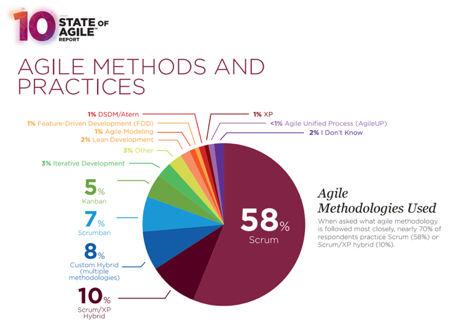
\includegraphics[width=16cm]{comparatif.png}
	\caption{Comparatif des méthodes agiles.}
	\label{fig:sp0}
\end{figure}

D’après la figure ci-dessus, Scrum est la méthodologie se basant sur les préceptes agiles la plus utilisés dans le monde. Il s’agit d’un recueil de bonne pratique, de définition de rôle et de cérémonies récurrentes rythmant le projet.
\begin{enumerate}
	\item  \textbf{Présentation de Scrum}.
	La méthodologie Scrum a été conçue pour améliorer grandement la productivité dans les équipes auparavant paralysés par des méthodologies plus lourdes. Le principe de base de Scrum est de focaliser l’équipe de façon itérative sur un ensemble de fonctionnalités à réaliser, dans des itérations de durée fixe allant d’une à quatre semaines, appelées SPRINT. 
	
Chaque sprint possède un but à atteindre, défini par le directeur de produit, à partir duquel sont choisies les fonctionnalités à implémenter dans le sprint. Un sprint aboutit toujours sur la livraison d’un produit partiel fonctionnel. Pendant ce temps, le Scrum Master a la charge de réduire au maximum les perturbations extérieurs et de résoudre les problèmes non techniques de l’équipe. Ce processus est illustré par la figure suivante 

\begin{figure}[H]
	\centering
	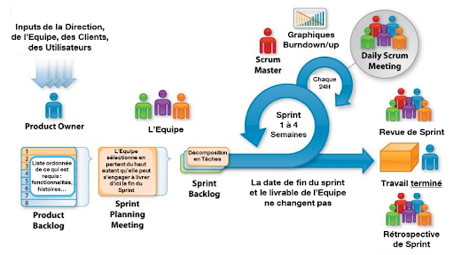
\includegraphics[width=16cm]{processus_scrum.png}
	\caption{Processus SCRUM.}
	\label{fig:sp0}
\end{figure}
\end{enumerate}
	  \textbf{Les acteurs}.
	
	On distingue plusieurs acteurs, dont : 
Le directeur de produit product owner est le représentant des clients et des utilisateurs, et fait également parti de l’équipe. 

Le ScrumMaster veille à l'application de la méthodologie Scrum au sein de l’équipe. 

L’équipe qui contribue à la réalisation des fonctionnalités du projet (planification, développement, test et documentation). A noter que les membres de l’équipe travaillent tous ensemble : Chaque membre peut faire ainsi des propositions, exprimer idées et écoute les autres.

	\textbf{Le processus}.

Tous les critères ou exigences du produits sont regroupées dans les journaux ou backlogs dont on distingue 2 types : 

\begin{itemize}[label=\textbullet, font=\LARGE \color{blue}] 
	\item  Le backlog de produit ou « Product backlog » qui regroupe la liste de fonctionnalités du produit.
	\item  Le backlog de sprint ou « Sprint backlog » en fonction des fonctionnalités du produit, regroupe la liste des tâches qui devra être réalisées à l’itération en cours. Chaque tâche aurait fait l’objet d’une estimation préalable de charge par l’ensemble des membres de l’équipe afin d’estimer au mieux les taches qui peuvent réaliser un sprint.
\end{itemize}

	\textbf{La planification}.
	
Le sprint : Dès le début d’un projet, la première planification permet de définir le périmètre de chaque itération appelé sprint. Chaque sprint dure quelques semaines et regroupe une liste de taches (défini dans le backlog).
 
La mêlée quotidienne : De plus, elle est rythmée par ce qu’on appelle une mêlée quotidienne d’un quart d’heure qui consiste chaque jour avec les membres de l’équipe ainsi que le directeur de produit de se tenir au courant de l’avancement du projet, notamment en : 

\begin{itemize}[label=\textbullet, font=\LARGE \color{blue}] 
	\item  Faisant le point sur le travail effectué la veille par chacun 
	\item  Définissant les taches qui sont réalisées durant la journée
	\item  Résolvant les éventuels problèmes qui avaient ou qui pourraient être rencontré par chacun 
	\item  Le développement suit un processus itératif et incrémental : de nouvelles fonctionnalités sont rajoutées au produit
	\item  Lean Development
	\item  Scrum
\end{itemize}

\textbf{La revue du sprint}.

La fin d’un sprint aboutit à la réalisation d’un produit avec des fonctionnalités partielles avec la documentation associée. Dans la plupart des cas, cela conduit à une revue de sprint consistant à faire une démonstration de la réalisation du sprint devant le client afin de valider le travail réalisé et d’avoir un retour pour éventuellement ajuster le backlog du produit.

\section{Modèle.}

Modéliser consiste à créer une représentation virtuelle d’une réalité de manière à faire ressortir les points auxquelles on s’intéresse, dans notre domaine, deux approches se démarquent : MERISE et UML

\begin{table}[H]
	\caption{Comparaison entre Merise et UML}
	\label{Comparaison entre Merise et UML}
	\centering
	\begin{tabularx}{\linewidth}{|X|X|}
		\hline \rowcolor{lightgray}  
		\textbf  \textbf{MERISE} & \textbf{UML}\\
		\hline
		 Méthode d'analyse et de conception d'un système d'information &  Langage de représentation d'un SI.\\
		\hline
		Méthode de modélisation de données et traitements orienté bases de données relationnelles &  Système de notation orienté objet\\
		\hline
		 relationnel  & Objet \\
		\hline
		 Franco-Français &  Internationale \\	
		\hline
		 Schéma directeur, étude préalable, étude détaillée et la réalisation &  Langage de modélisation des systèmes standards, qui utilise des diagrammes pour représenter chaque aspect d'un système : statique, dynamique. En s'appuyant sur la notion d'orienté objet. \\	
		\hline		
	\end{tabularx}
\end{table}

\subsection{Choix du langage de modélisation.\cite{Ref02}}

UML est un langage de modélisation graphique à base de pictogrammes, conçu pour représenter, spécifier les artefacts de systèmes logiciels. Il est destiné à comprendre et décrire des besoins spécifiés et documentés des systèmes, esquissé des architectures logicielles. Ce langage de modélisation comble une lacune importante des technologies objet, il permet d’exprimer, d’élaborer et de modéliser au sens de la théorie des langages, de ce fait il contient les éléments constitutifs de ce derniers : concepts, syntaxe et sémantique. La puissance et l’intérêt d’UML est qu’il normalise la sémantique des concepts qu’il véhicule, il repose sur un méta modèle pour permettre à n’importe qui de déchiffrer son intention de manière non équivoque, il est donc primordiale de s’accorder sur la sémantique des éléments de modélisation, bien avant de s'intéresser à la manière de les présenter.

Les points forts suivant sont ceux ayant motiver notre choix :

\begin{itemize}[label=\textbullet, font=\LARGE \color{blue}] 
	\item  Gain de précision
	\item  Gage de stabilité
	\item  Utilisation d'outils
	\item  Il cadre l'analyse et facilite la compréhension de représentations abstraites complexes.
\end{itemize}

Son caractère polyvalent et sa souplesse en font un langage universel.
 

\section{Concept d'UML}

\subsection{Définition}

Langage de modélisation unifié « Unified Modeling Language » est un langage de modélisation graphique à base de pictogrammes. Il est apparu dans le monde du génie logiciel, dans le cadre de la « conception orientée objet ». Couramment utilisé dans les projets logiciels, il peut être appliqué à toutes sortes de systèmes ne se limitant pas au domaine informatique.

\subsection{Unité}

UML est utilisé pour spécifier, visualiser, modifier et construire les documents nécessaires au bon développement d’un logiciel orienté objet. UML offre un standard de modélisation, pour représenter l’architecture de logicielle. Les différents éléments représentables sont « Activité d’un objet/logiciel, Acteurs, Processus, Schéma de base de données, Composants logiciels et Réutilisation de composants ». Grâce aux outils de modélisation UML, il est également possible de générer automatiquement une partie de code, par exemple en langage Java, à partir des divers documents réalisés.

\subsection{Présentation de quelques diagrammes UML}

 \textbf{Diagramme de cas d'utilisation}

Les cas d’utilisation constituent un moyen de recueillir et de décrire les besoins des acteurs du système. Ils peuvent être aussi utilisés ensuite comme moyen d’organisation du développement du logiciel, notamment pour la structuration et le déroulement des tests du logiciel. Un cas d’utilisation permet de décrire l’interaction entre les acteurs (utilisateurs du cas) et le système. La description de l’interaction est réalisée suivant le point de vue de l’utilisateur. La représentation d’un cas d’utilisation met en jeu trois concepts : l’acteur, le cas d’utilisation et l’interaction entre l’acteur et le cas d’utilisation.

\begin{itemize}[label=\textbullet, font=\LARGE \color{blue}] 
	\item   \textbf{Acteur :} 
	Un acteur est un utilisateur type qui a toujours le même comportement vis-à-vis d’un cas d’utilisation. Ainsi les utilisateurs d’un système appartiennent à une ou plusieurs classes d’acteurs selon les rôles qu’ils tiennent par rapport au système. Un acteur peut aussi être un système externe avec lequel le cas d’utilisation va interagir. Un acteur peut se représenter symboliquement par un bonhomme et être identifié par son nom. 
	
	\item  \textbf{Cas d'utilisation et interaction :}
		\begin{itemize}[label=\textbullet, font=\LARGE \color{black}] 
			\item  Un cas d’utilisation correspond à un certain nombres d’actions que le système devra exécuter en réponse à un besoin d’un acteur. Un cas d’utilisation doit produire un résultat observable pour un ou plusieurs acteurs ou parties prenantes du système.
			\item  Une interaction permet de décrire les échanges entre un acteur et un cas d’utilisation.
		\end{itemize}
	\item  \textbf{Relations entre cas d'utilsiation :}
	Afin d’optimiser la formalisation des besoins en ayant recours notamment à la réutilisation de cas d’utilisation, trois relations peuvent être décrites entre cas d’utilisation : une relation d’inclusion (include), une relation d’extension (extend) et une relation de généralisation. 
\end{itemize}

\textbf{Diagramme de séquences}

L’objectif du diagramme de séquence est de représenter les interactions entre objets en indiquant la chronologie des échanges. Cette représentation peut se réaliser par cas d’utilisation en considérant les différents scenarios associés. 
		\begin{itemize}[label=\textbullet, font=\LARGE \color{blue}] 
			\item   \textbf{Ligne de vie :} 
		
			Une ligne de vie représente l’ensemble des opérations exécutées par un objet. Un message reçu par un objet déclenche l’exécution d’une opération. Le retour d’information peut être implicite (cas général) ou explicite à l’aide d’un message de retour. 
			\item  \textbf{Message synchrone et asynchrone :} 
					\begin{itemize}[label=\textbullet, font=\LARGE \color{black}] 
						\item  Message synchrone – dans ce cas, l’émetteur reste en attente de la réponse à son message avant de poursuivre ses actions. La flèche avec extrémité pleine symbolise ce type de message. Le message retour peut ne pas être représenté car il est inclus dans la fin d’exécution de l’opération de l’objet destinataire du message.
						\item  Message asynchrone – dans ce cas, l’émetteur n’attend pas la réponse à son message, il poursuit l’exécution de ses opérations. C’est une flèche avec une extrémité non pleine qui symbolise ce type de message. 
					\end{itemize}
		\end{itemize}
		
UML possède plus de diagramme que celles présenté ci-haut. Nous ne pouvons pas les présenter tous dans ce mémoire, de peur que cela soit long et que beaucoup de livre explique déjà toutes ses notions de façon claire avec des exemples à l’appui. Pour plus d’information, nous conseillons la consultation des livres UML, Analyse et Conception et UML 2 pour les développeurs qui ont été notre principale source d’inspiration dans cette partie. 

\textbf{Diagramme de classes}
Le diagramme de classe constitue l’un des pivots essentiels de la modélisation avec UML. En effet ce diagramme permet de donner la représentation statique du système à développer. Cette représentation est centrée sur les concepts de classe et d’association. Chaque classe se décrit par les données et les traitements dont elle est responsable pour elle-même et vis-à-vis des autres classes. Les traitements sont matérialisés par des opérations.

La description du diagramme de classe est fondée sur :

\begin{itemize}[label=\textbullet, font=\LARGE \color{blue}] 
	\item  Le concept d'objet
	
	Un objet est un concept, une abstraction ou une chose qui a un sens dans le contexte du système à modéliser. Chaque objet a une identité et peut être distingué des autres sans considérer à priori les valeurs de ses propriétés.
Un objet est caractérisé par les valeurs de ses propriétés qui lui confèrent des états significatifs suivant les instants considérés.

	\item  Le concept de classe comprenant les attributs et les opération
	
	Une classe décrit un groupe d’objets ayant les mêmes propriétés (attributs), un même comportement (opérations), et une sémantique commune (domaine de définition). Un objet est une instance d’une classe. La classe représente l’abstraction de ses objets. Au niveau de l’implémentation, c’est-à-dire au cours de l’exécution d’un programme, l’identificateur d’un objet correspond à une adresse mémoire.
	
	\item  Les différents types d'association entre classes.
	
	La généralisation est la relation entre une classe et deux autres classes ou plus partageant un sous-ensemble commun d’attributs et/ou d’opérations.
La classe qui est affinée s’appelle superclasse, les classes affinées s’appellent sous-classes. L’opération qui consiste à créer une superclasse à partir de classes s’appelle généralisation. Inversement la spécialisation consiste à créer des sous-classes à partir d’une classe.

\end{itemize}

\section{Analyse et Modélisation}

\subsection{Les acteurs système}

Un acteur représente un rôle joué par une entité externe (utilisateur humain, dispositif matériel ou autre système) qui interagit directement avec le système étudié. Il peut consulter et/ou modifier directement l’état du système. Les acteurs qui interagissent avec l’application à concevoir sont :

\begin{itemize}[label=\textbullet, font=\LARGE \color{blue}] 
	\item  Le responsable du content-writer : consultation de l’application, modification des doubles bannières, modification des sliders de l’application 
	\item  Le responsable marketing : consultation de l’application, la création, modification des notifications push, la création/modification des pop-ups
	\item  Le client : consultation de l’application
	\item  L’informaticien : paramétrage de l’application et création des différents utilisateurs
	\item  Le responsable de la planification commerciale : consultation de l’application, la mise en place des bloc produits et catégories
\end{itemize}

\subsection{Les cas d'utilisation}

\textbf{Identification des cas d’utilisation :}

Un cas d’utilisation définit une manière d’utiliser le système et permet d’en décrire les exigences fonctionnelles. Chaque cas d’utilisation contient un ou plusieurs scénarios qui définissent comment le système devrait interagir avec les utilisateurs (appelés acteurs) pour atteindre un but ou une fonction spécifique d’un travail. Un acteur d’un cas d’utilisation peut être un humain ou un autre système externe à celui que l’on tente de définir.

Lors de notre analyse des besoins nous avons pu identifier les actions importantes que nous présenterons ci-dessous et nous les modélisons par la suite avec les diagrammes cas d’utilisations d’UML.

\begin{table}[H]
	\caption{Acteurs du système.\cite{Ref8}}
	\label{Acteurs du système.}
	\centering
	\begin{tabularx}{\linewidth}{|X|X|X|}
		\hline \rowcolor{lightgray}  
		\textbf{Cas d'utilisation} & \textbf{Acteurs} & \textbf{Opérations}\\
		\hline
		Authentification & Tous les utilisateurs &  Connexion, Déconnexion\\
		\hline
		Gestion des sliders & Responsable content-writer &  Ajouter, Modifier, Supprimer, Consulter\\
		\hline
		Gestion des doubles bannières & Responsable content-writer  & Ajouter, Modifier, Supprimer, Consulter\\
		\hline
		Gestion des blocs produits  & Responsable de la planification commercial &  Ajouter, Modifier, Supprimer, Consulter \\	
		\hline
		Gestion des push notification & Responsable marketing  & Ajouter, Modifier, Supprimer, Consulter\\
		\hline
		Gestions des paramètres  & Informaticien & Ajouter, Modifier, Supprimer, Consulter\\
		\hline
		Gestion des utilisateurs & Informaticien & Ajouter, Modifier, Supprimer, Consulter \\
		\hline
	\end{tabularx}
\end{table}

\textbf{\underline{Identification des cas d’utilisation :}}

Le diagramme de cas d’utilisation est le diagramme UML utilisés pour donner une vision globale du comportement fonctionnel d’un système logiciel. Ils sont utiles pour des présentations auprès de la direction ou des acteurs d’un projet, mais pour le développement, les cas d’utilisation sont plus appropriés.

\begin{figure}[H]
	\centering
	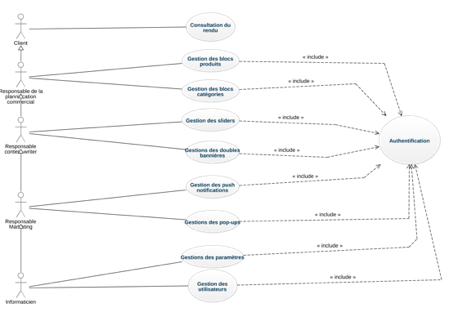
\includegraphics[width=16cm]{use_case.png}
	\caption{Diagramme de cas d'utilisation du système.}
	\label{fig:use_cas}
\end{figure}

\textbf{\underline{Description de quelques cas d'utilisation :}}

Nous allons désormais parler de l’interaction entre les acteurs et le système : il s’agit de décrire la chronologie des actions qui devront être réalisées par les acteurs et par le système lui-même. On parle d’ailleurs de scénarios. 

\begin{enumerate}
	\item  \textbf{Description du cas d'utilisation "Gestion des blocs produits"}.
	
	\begin{table}[H]
	\caption{Description du cas d'utilisation "Gestion des blocs produits"}
	\label{Description du cas d'utilisation "Gestion des blocs produits"}
	\centering
	\begin{tabularx}{\linewidth}{|X|X|}
		\hline \rowcolor{lightgray}  
		\textbf  \textbf{ } & \textbf{Description}\\
		\hline
		 Titre &  Gestion des blocs produits\\
		\hline
		But & Il permet de mettre sur la page d'accueil les produits voulu afin de présenter une variété de produits à un utilisateur\\
		\hline
		 Acteur  & Responsable de la planification commercial \\
		\hline
		 Pré conditions &  L'utilisateur doit s'authentifier \\	
		\hline		
		 Enchainement &  L'utilisateur s'authentifie, L'utilisateur demande d'ajouter, modifier ou supprimer les produits mis en avant, le système affiche le formulaire ou la liste des produits, le système verifie la validité des données, enregistre et confirme \\	
		\hline			
		 Alternative & le système affiche un message d'erreur lorsque l'utilisateur fournit des données incomplètes ou erronées ( ajout et modification) \\	
		\hline			
	\end{tabularx}
\end{table}

\item  \textbf{Description du cas d'utilisation "Gestion des doubles bannieres"}.

	\begin{table}[H]
	\caption{Description du cas d'utilisation "Gestion des doubles bannieres"}
	\label{Description du cas d'utilisation "Gestion des doubles bannieres"}
	\centering
	\begin{tabularx}{\linewidth}{|X|X|}
		\hline \rowcolor{lightgray}  
		\textbf  \textbf{ } & \textbf{Description}\\
		\hline
		 Titre &  Gestion des doubles bannieres\\
		\hline
		But & Il permet de mettre sur la page d'accueil les doubles bannieres voulu afin de présenter une variété de catégories et ou boutiques officielles à un utilisateur\\
		\hline
		 Acteur  & Responsable content-writer \\
		\hline
		 Pré conditions &  L'utilisateur doit s'authentifier \\	
		\hline		
		 Enchainement &  L'utilisateur s'authentifie, L'utilisateur demande d'ajouter, modifier ou supprimer les produits mis en avant, le système affiche le formulaire ou la liste des doubles bannieres, le système verifie la validité des données, enregistre et confirme \\	
		\hline			
		 Alternative & le système affiche un message d'erreur lorsque l'utilisateur fournit des données incomplètes ou erronées ( ajout et modification) \\	
		\hline			
	\end{tabularx}
\end{table}


\item  \textbf{Description du cas d'utilisation "Gestion des push notifications"}.

	\begin{table}[H]
	\caption{Description du cas d'utilisation "Gestion des push notifications"}
	\label{Description du cas d'utilisation "Gestion des push notifications"}
	\centering
	\begin{tabularx}{\linewidth}{|X|X|}
		\hline \rowcolor{lightgray}  
		\textbf  \textbf{ } & \textbf{Description}\\
		\hline
		 Titre &  Gestion des push notifications\\
		\hline
		But & Il permet d’effectuer les notifications sur l’application des utilisateurs afin de les annonces nos meilleurs deals ou nos promotions\\
		\hline
		 Acteur  & Responsable Responsable marketing \\
		\hline
		 Pré conditions &  L'utilisateur doit s'authentifier \\	
		\hline		
		 Enchainement &  L'utilisateur s'authentifie, L'utilisateur demande d'ajouter, modifier ou supprimer les produits mis en avant, le système affiche le formulaire ou la liste des push notifications, le système verifie la validité des données, enregistre et confirme \\	
		\hline			
		 Alternative & le système affiche un message d'erreur lorsque l'utilisateur fournit des données incomplètes ou erronées ( ajout et modification) \\	
		\hline			
	\end{tabularx}
\end{table}

\item  \textbf{Description du cas d'utilisation "Gestion des sliders"}.

	\begin{table}[H]
	\caption{Description du cas d'utilisation "Gestion des sliders"}
	\label{Description du cas d'utilisation "Gestion des sliders"}
	\centering
	\begin{tabularx}{\linewidth}{|X|X|}
		\hline \rowcolor{lightgray}  
		\textbf  \textbf{ } & \textbf{Description}\\
		\hline
		 Titre &  Gestion des sliders\\
		\hline
		But & Il permet de mettre sur la page d’accueil les sliders pour présenter nos multiples catégories et ou boutiques officielles  \\
		\hline
		 Acteur  & Responsable Responsable content-writer \\
		\hline
		 Pré conditions &  L'utilisateur doit s'authentifier \\	
		\hline		
		 Enchainement &  L'utilisateur s'authentifie, L'utilisateur demande d'ajouter, modifier ou supprimer les produits mis en avant, le système affiche le formulaire ou la liste des sliders, le système vérifie la validité des données, enregistre et confirme \\	
		\hline			
		 Alternative & le système affiche un message d'erreur lorsque l'utilisateur fournit des données incomplètes ou erronées ( ajout et modification) \\	
		\hline			
	\end{tabularx}
\end{table}
\end{enumerate}

\subsection{Modélisations Conceptuelles}

\textbf{\underline{Diagramme de séquence.}}.

Les diagrammes de séquences permettent décrire comment les éléments du système interagissent entre eux et avec les acteurs. Les objets au cœur d’un système interagissent en s’échangeant des messages. Les acteurs interagissent avec le système au moyen d’IHM (Interfaces Homme-Machine).

\underline{Quelques diagrammes de séquence de l’application.}

\begin{enumerate}
	\item  \underline{Diagramme de séquence "S'authentifier"}.
\begin{figure}[H]
	\centering
	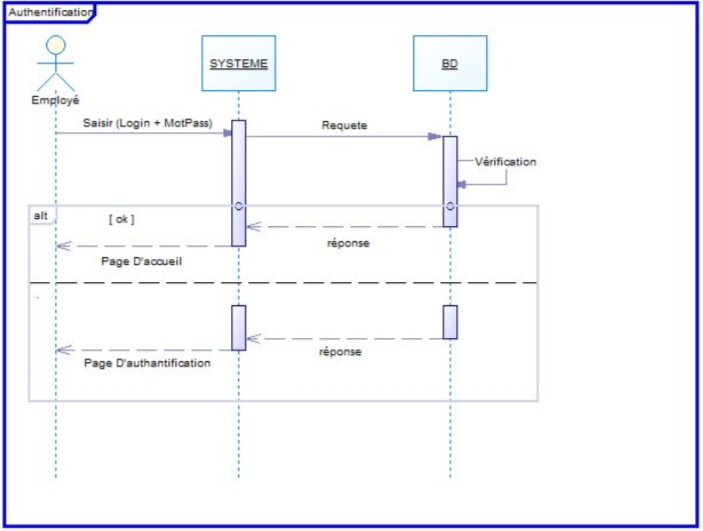
\includegraphics[width=18cm]{authentification.png}
	\caption{Diagramme de séquence d'authentification.}
	\label{fig:sp0}
\end{figure}

\item  \underline{Diagramme de séquence "Gestion des doubles bannières"}.
\begin{figure}[H]
	\centering
	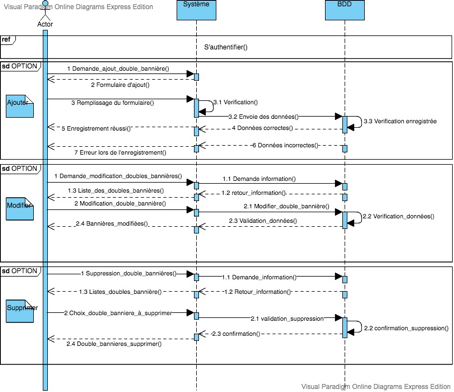
\includegraphics[width=18cm]{seq.png}
	\caption{Diagramme de séquence "Gestion des doubles bannières".}
	\label{fig:sp0}
\end{figure}

\item  \underline{Diagramme de séquence "sliders"}.
\begin{figure}[H]
	\centering
	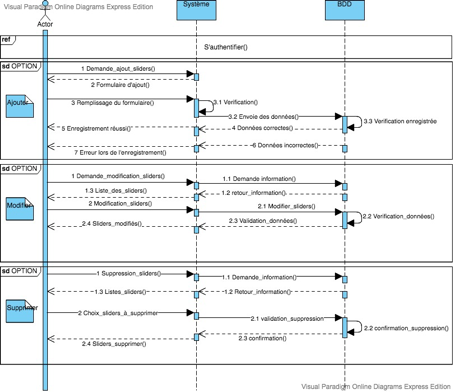
\includegraphics[width=18cm]{slider.png}
	\caption{Diagramme de séquence "sliders".}
	\label{fig:sp0}
\end{figure}

\item  \underline{Diagramme de séquence "Gestion des push notifications"}.
\begin{figure}[H]
	\centering
	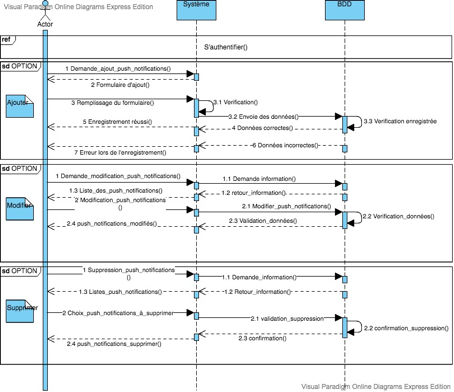
\includegraphics[width=18cm]{push.png}
	\caption{Diagramme de séquence "Gestion des push notifications".}
	\label{fig:sp0}
\end{figure}
\end{enumerate}

\textbf{\underline{Diagramme de classe.}}.

Un diagramme de classes UML décrit les structures d’objets et d’informations utilisées par votre application, à la fois en interne et dans la communication avec ses utilisateurs. Il décrit les informations sans faire référence à une implémentation particulière. Ses classes et relations peuvent être implémentées de nombreuses manières, comme les tables de bases de données, les nœuds XML ou encore les compositions d’objets logiciels.

Pour un soucis de confidentialité il m'a été demandé de ne présenter que les classes qui interviennent avec mon mémoire.

\begin{figure}[H]
	\centering
	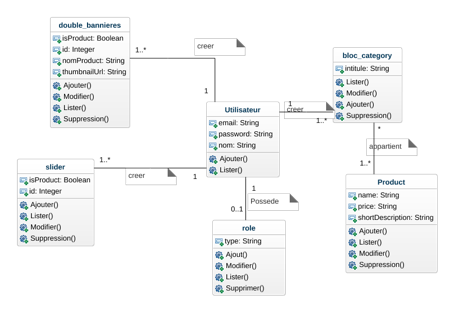
\includegraphics[width=18cm]{classe.png}
	\caption{Diagramme de classe .}
	\label{fig:sp0}
\end{figure}

\textbf{\underline{Diagramme de déploiement.}}.

Le diagramme de déploiement est une vue statique qui sert à représenter l’utilisation de l’infrastructure physique par le système et la manière dont les composants du système sont répartis ainsi que la relation entre eux.

\begin{figure}[H]
	\centering
	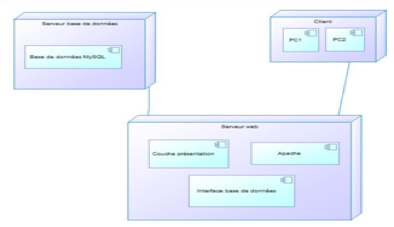
\includegraphics[width=14cm]{deploiement.png}
	\caption{Diagramme de deploiement.}
	\label{fig:sp0}
\end{figure}

\section{Architecture générale de l'application}
\subsection{Définition}

Il existe plusieurs types d’architectures, parmi lesquelles :
\begin{enumerate}
	\item  \underline{L'architecture 2-tiers :}
	L’architecture à deux niveaux (aussi appelée architecture 2-tier, tiers signifiant rangée en anglais) caractérise les systèmes clients/serveurs pour lesquels le client demande une ressource et le serveur la lui fournit directement, en utilisant ses propres ressources. Cela signifie que le serveur ne fait pas appel à une autre application afin de fournir une partie du service
	\begin{figure}[H]
	\centering
	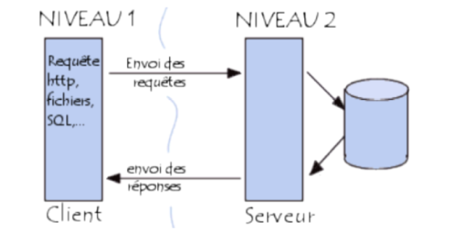
\includegraphics[width=14cm]{2-tiers.png}
	\caption{Architecture 2-tiers.}
	\label{fig:sp0}
\end{figure}


\item  \underline{L'architecture 3-tiers :}
	Dans l’architecture à 3 niveaux ( appelée architecture 3-tiers), il existe un niveau intermédiaire, c’est-à-dire que l’on a généralement une architecture partagée entre :
	
	\begin{itemize}[label=\textbullet, font=\LARGE \color{blue}] 
	\item  Client : c’est-à-dire l’ordinateur demandeur de ressources, équipée d’une interface utilisateur (généralement un navigateur web) chargée de la présentation
	\item  Le serveur d’application ( appelé également middleware), chargé de fournir la ressource mais faisant appel à un autre serveur
	\item  Le serveur de données, fournissant au serveur d’application les données dont il a besoin 
\end{itemize}

	\begin{figure}[H]
	\centering
	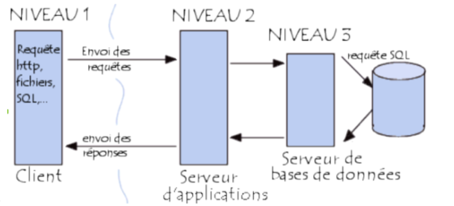
\includegraphics[width=14cm]{3-tiers.png}
	\caption{Architecture 3-tiers.}
	\label{fig:sp0}
\end{figure}


\item  \underline{L'architecture N-tiers :}
	Dans l’architecture à 3 niveau, chaque serveur ( niveau 2 et 3 ) effectue une tâche (un service) spécialisée. Un serveur peut donc utiliser les services d’un ou plusieurs autres serveurs afin de fournir son propre service. Par conséquent, l’architecture à trois niveaux est potentiellement une architecture à N niveaux.
	
	\begin{figure}[H]
	\centering
	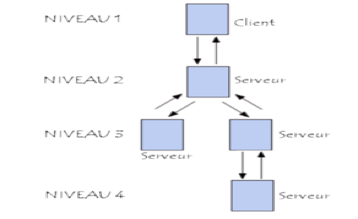
\includegraphics[width=14cm]{n-tiers.png}
	\caption{Architecture N-tiers.}
	\label{fig:sp0}
\end{figure}
\end{enumerate}

\subsection{Architecture de notre système}

Dans notre cas, il s’agit d’une architecture 3-tiers, c’est-à-dire à 3 niveaux :

	\begin{itemize}[label=\textbullet, font=\LARGE \color{blue}] 
	\item  Le niveau 1 : il s’agit de l’interface utilisateur où sera lancée une requête.
	\item  Le niveau 2 : il s’agit dans notre cas du serveur de l’établissement
	\item  Le niveau 3 : il s’agit du serveur SQL Server
\end{itemize}

Tout système d’information nécessite la réalisation de trois groupes de fonctions : le stockage des données, la logique applicative et la présentation. Ces trois parties sont indépendantes les unes des autres : on peut ainsi vouloir modifier la présentation sans modifier la logique applicative. La conception de chaque partie doit également être indépendante, toutefois la conception de la couche la plus basse est utilisée dans la couche d’au-dessus.

Dans ce chapitre nous avons présenté d’une façon globale, les deux étapes essentielles du système élaboré pour l’analyse et la conception de notre application en suivant le processus de normalisation UML et les différents diagrammes, afin de faciliter la phase de réalisation.
Le chapitre suivant, quant à lui, sera consacré à la phase de développement de notre application.








